\section{CGAN}
To implement a \gls{CGAN} it is only necessary to modify an existing \gls{GAN} to receive a conditional label. For these experiments, the same base used for the \gls{DCGAN} was used to construct the \gls{CGAN}, the only difference was the addition of another input for the label that will pass through an embedding layer and be incorporated into a channel of the other input, as discussed in \autoref{sub:cgan}.

\subsection{MNIST}
Training the \gls{CGAN} on the \gls{MNIST} dataset produced the results seen in \autoref{fig:cgan_mnist_metrics}.\begin{figure}[hbt]
    \centering
    \caption{Metrics when training a CGAN on MNIST}
    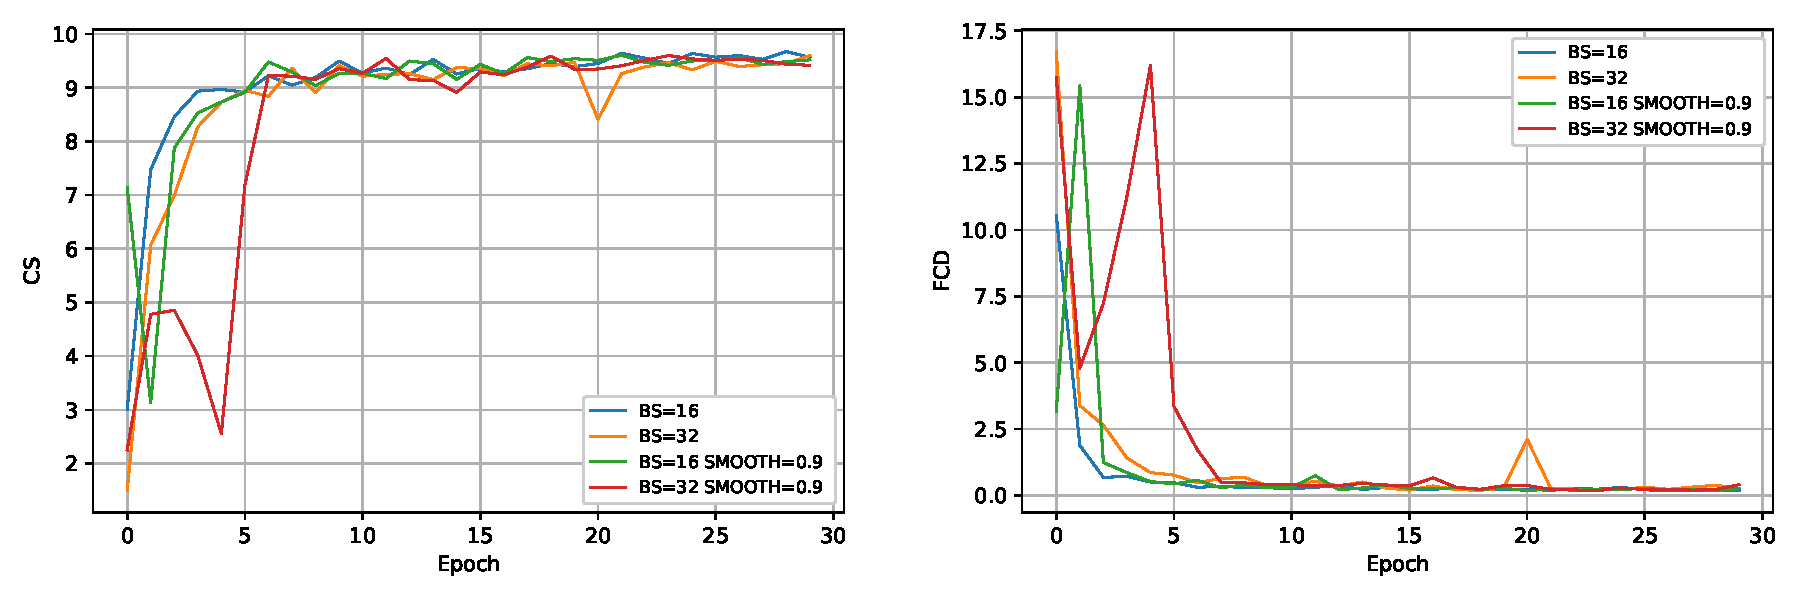
\includegraphics[width=\textwidth]{chapters/Experiments/CGAN/mnist_metrics.pdf}
    \fonte{From the author (2021)}
    \label{fig:cgan_mnist_metrics}
\end{figure}

These results show not only that the metrics have improved, but also that the training is much more stable, for all tests the training produced similar good results.

One of the main benefits of the \gls{CGAN} architecture is the fact that the resulting sample can be controlled by feeding the desired label to the generator. This can be seen in the samples produced by the best model (\texttt{BS=16 SMOOTH=0.9}) shown in \autoref{fig:cgan_mnist_samples}, where each row was conditioned to produce a different set of digits.
\begin{figure}[hbt]
    \centering
    \caption{Samples when training a CGAN on MNIST}
    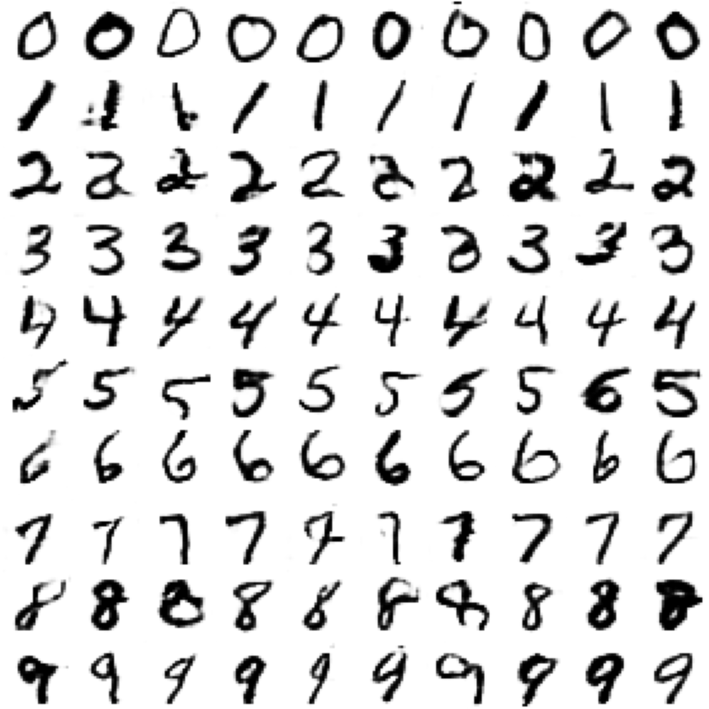
\includegraphics[width=0.5\textwidth]{chapters/Experiments/CGAN/mnist_samples.png}
    \fonte{From the author (2021)}
    \label{fig:cgan_mnist_samples}
\end{figure}


\subsection{Fashion MNIST}
Training the \gls{CGAN} on the Fashion MNIST dataset produced the results seen in \autoref{fig:cgan_fashion_metrics}.
\begin{figure}[hbt]
    \centering
    \caption{Metrics when training a CGAN on Fashion MNIST}
    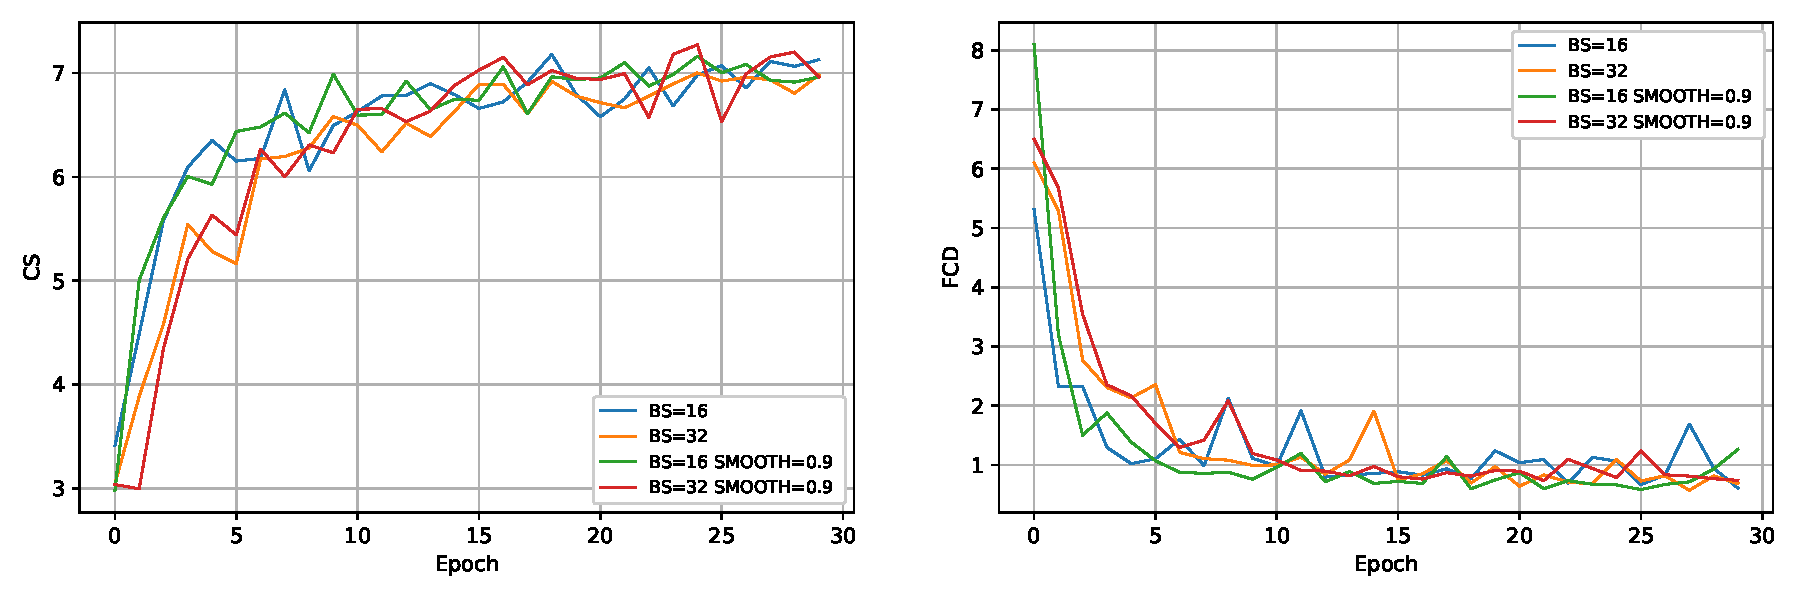
\includegraphics[width=\textwidth]{chapters/Experiments/CGAN/fashion_metrics.pdf}
    \fonte{From the author (2021)}
    \label{fig:cgan_fashion_metrics}
\end{figure}

The same behaviour seen for \gls{MNIST} can also be seen here, the overall quality increased, this time however the level of stability is not as strong. The samples produced by the best test (\texttt{BS=32}) are shown in \autoref{fig:cgan_fashion_samples}.
\begin{figure}[hbt]
    \centering
    \caption{Samples when training a CGAN on Fashion MNIST}
    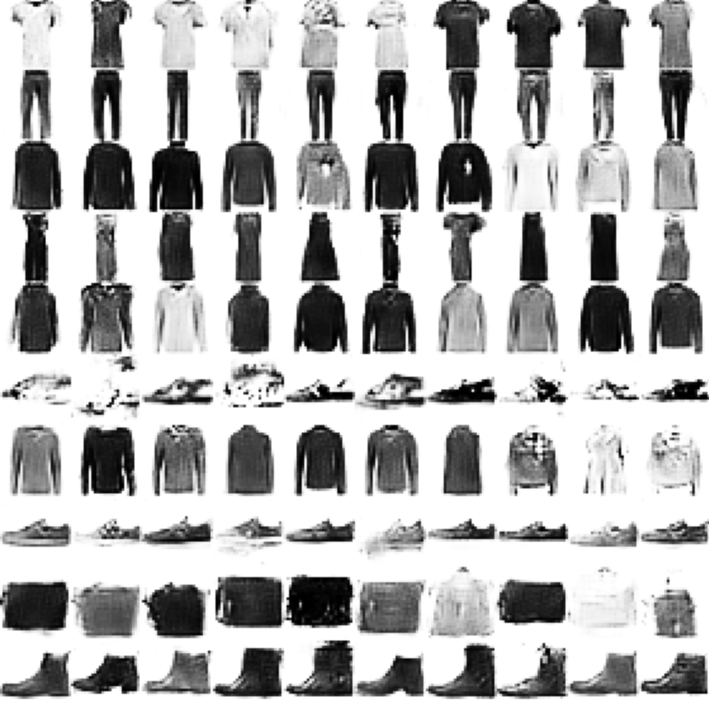
\includegraphics[width=0.5\textwidth]{chapters/Experiments/CGAN/fashion_samples.png}
    \fonte{From the author (2021)}
    \label{fig:cgan_fashion_samples}
\end{figure}


\subsection{CIFAR-10}
Training the \gls{CGAN} on the \gls{CIFAR}-10 dataset produced the results seen in \autoref{fig:cgan_cifar_metrics}. In these experiments it was also tested the \gls{beta_1} term of Adam to see if some momentum in the updates would be beneficial.
\begin{figure}[hbt]
    \centering
    \caption{Metrics when training a CGAN on CIFAR-10}
    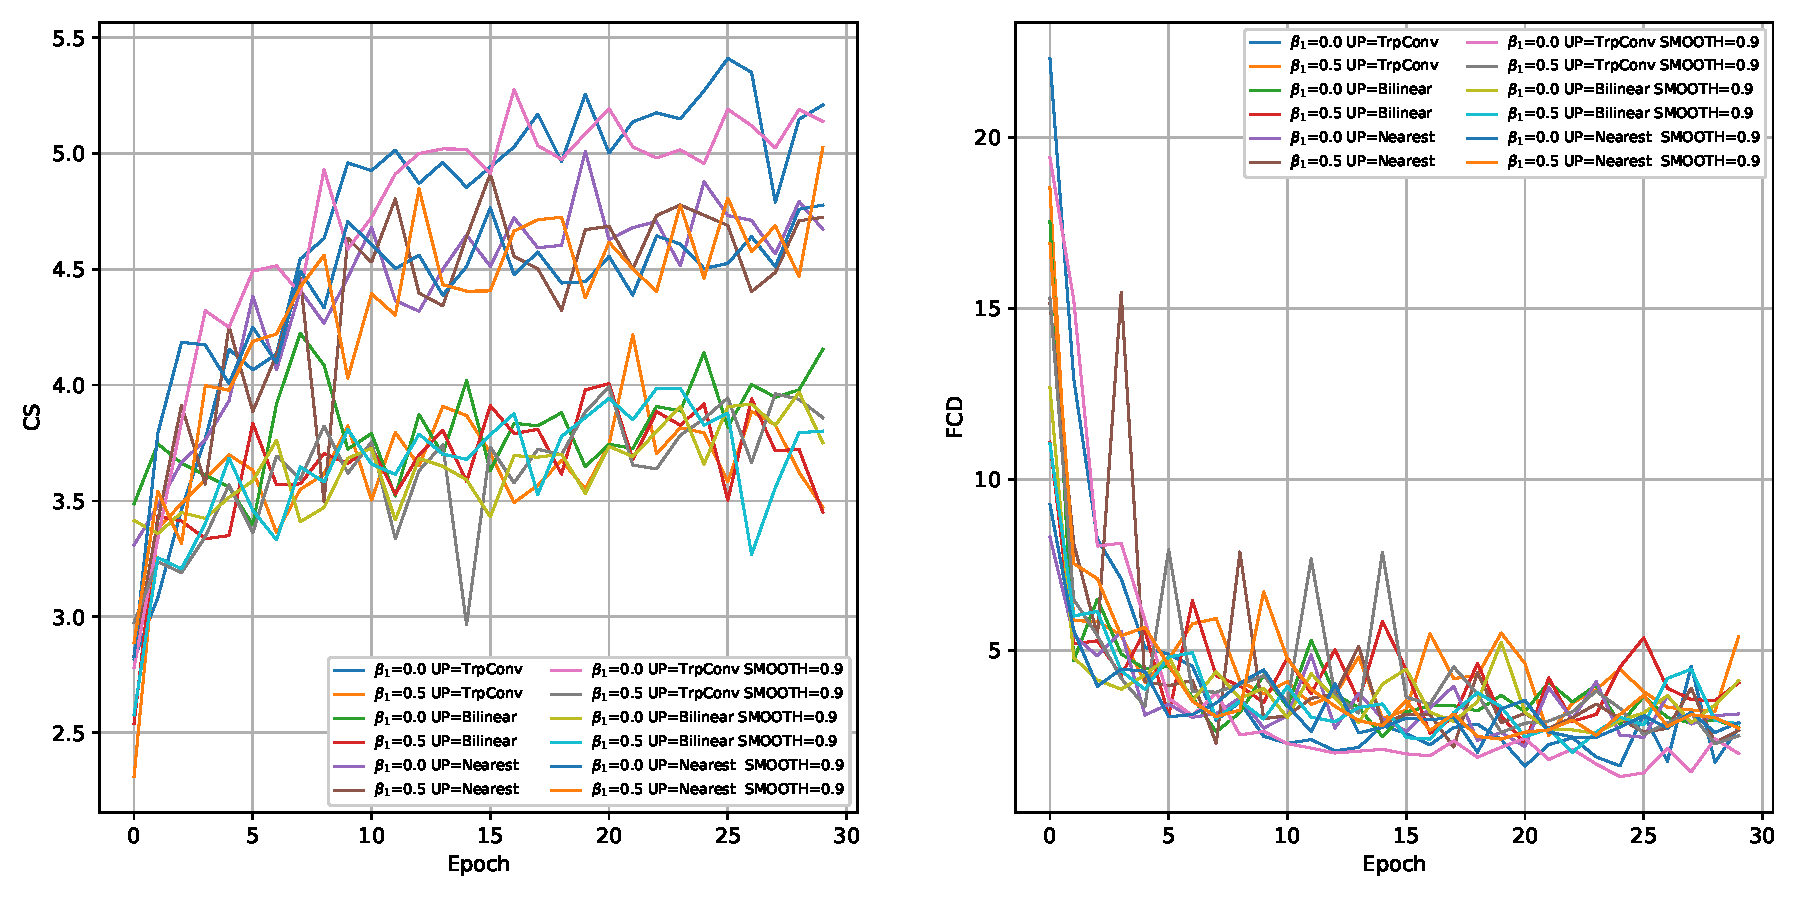
\includegraphics[width=\textwidth]{chapters/Experiments/CGAN/cifar_metrics.pdf}
    \fonte{From the author (2021)}
    \label{fig:cgan_cifar_metrics}
\end{figure}

To better understand how each component affects the results it is useful to highlight them separately. \autoref{fig:cgan_cifar_upsampling} shows how the metrics evolve for the different upsampling techniques. The same behaviour observed previously is also seen here, still the transposed convolutions perform better, followed by nearest neighbour and bilinear upsampling.
\begin{figure}[hbt]
    \centering
    \caption{Effects of upsampling when training a CGAN on CIFAR-10}
    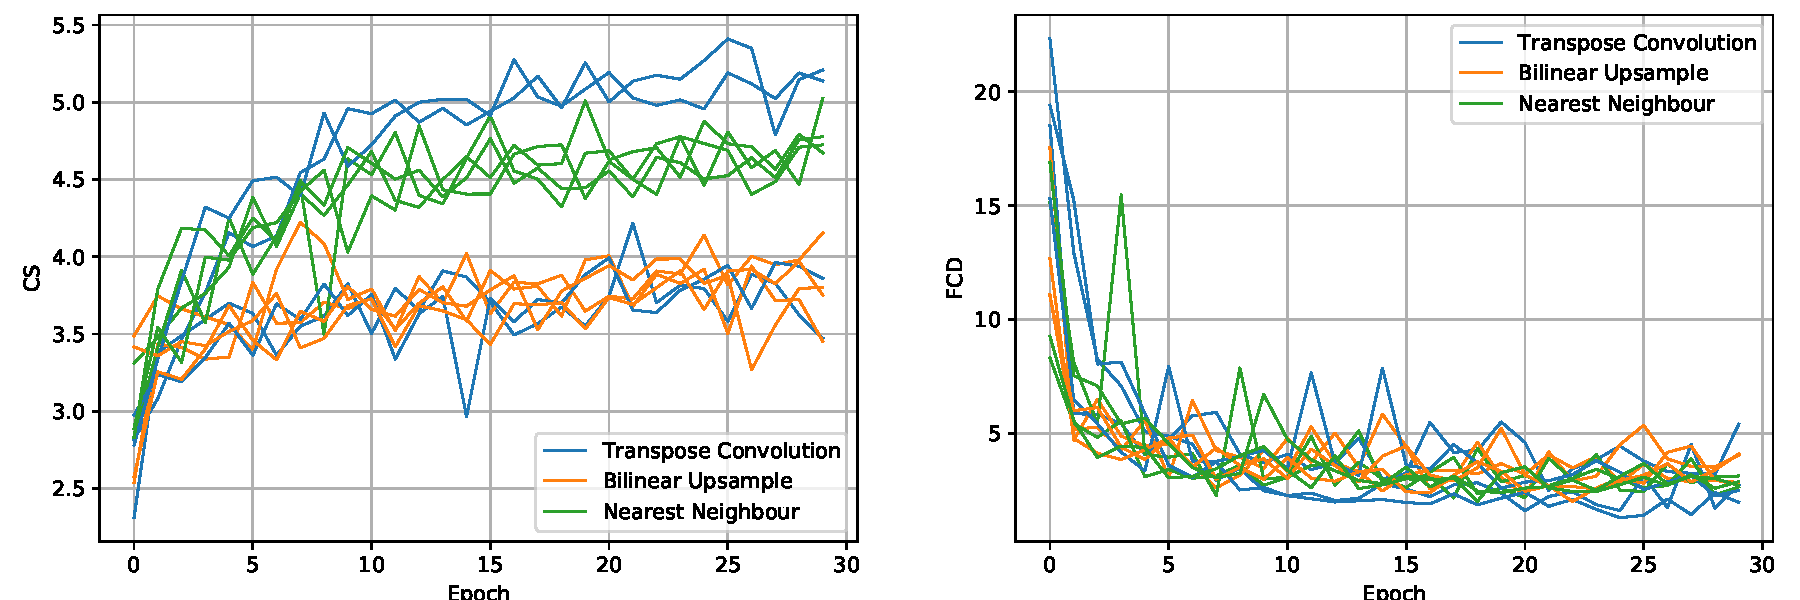
\includegraphics[width=\textwidth]{chapters/Experiments/CGAN/cifar_upsampling.pdf}
    \fonte{From the author (2021)}
    \label{fig:cgan_cifar_upsampling}
\end{figure}

In \autoref{fig:cgan_cifar_beta1} it is possible to see the effect of the momentum term \gls{beta_1} in training. The results support the idea that momentum does not help for \gls{CIFAR}-10. Also note how the bad performing cases of transposed convolutions seen in \autoref{fig:cgan_cifar_upsampling} are because the use of momentum.
\begin{figure}[hbt]
    \centering
    \caption{Effects of momentum when training a CGAN on CIFAR-10}
    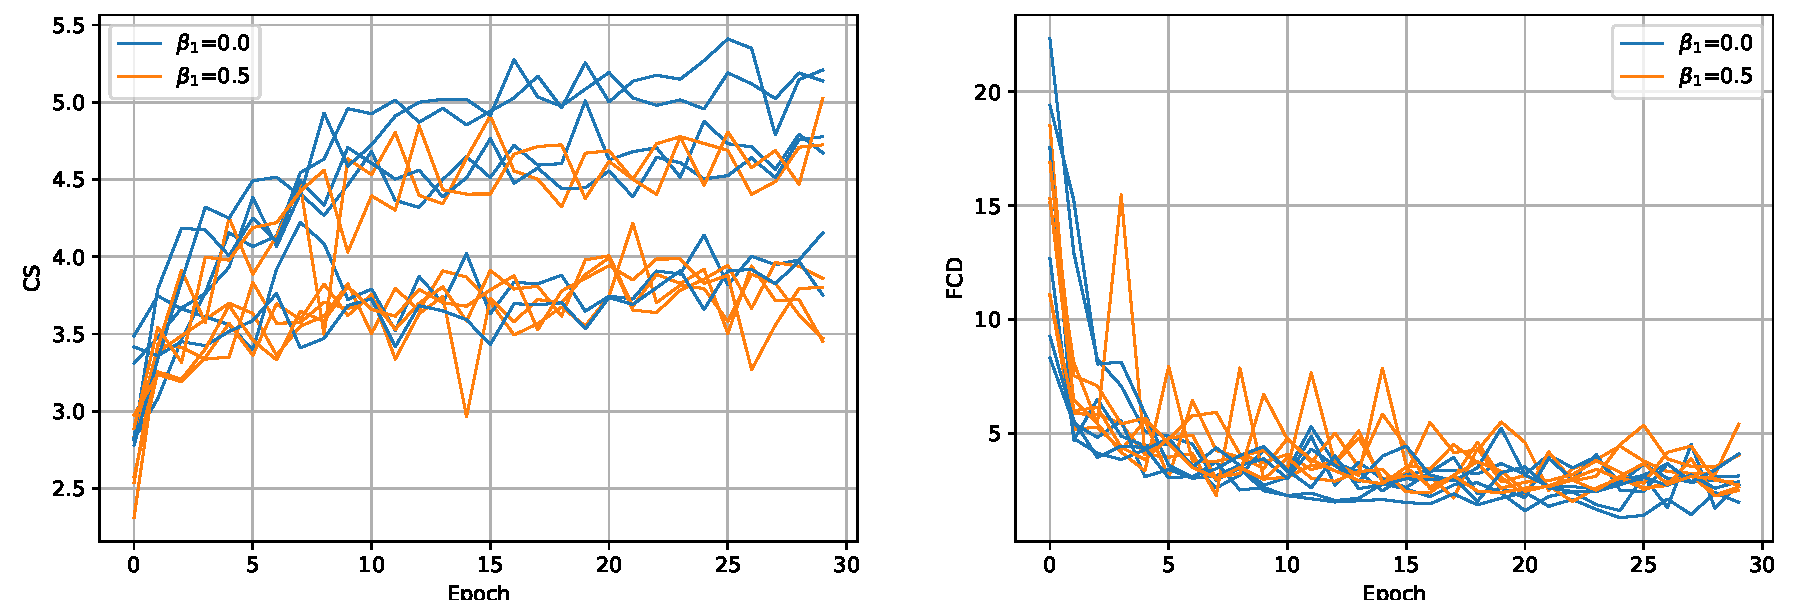
\includegraphics[width=\textwidth]{chapters/Experiments/CGAN/cifar_beta1.pdf}
    \fonte{From the author (2021)}
    \label{fig:cgan_cifar_beta1}
\end{figure}

Lastly, the effects of label smoothing can be seen in \autoref{fig:cgan_cifar_smoothing}. The impact is still not very significative, although it can be seen a small tendency for better values of the \gls{FCD}.
\begin{figure}[hbt]
    \centering
    \caption{Effects of label smoothing when training a CGAN on CIFAR-10}
    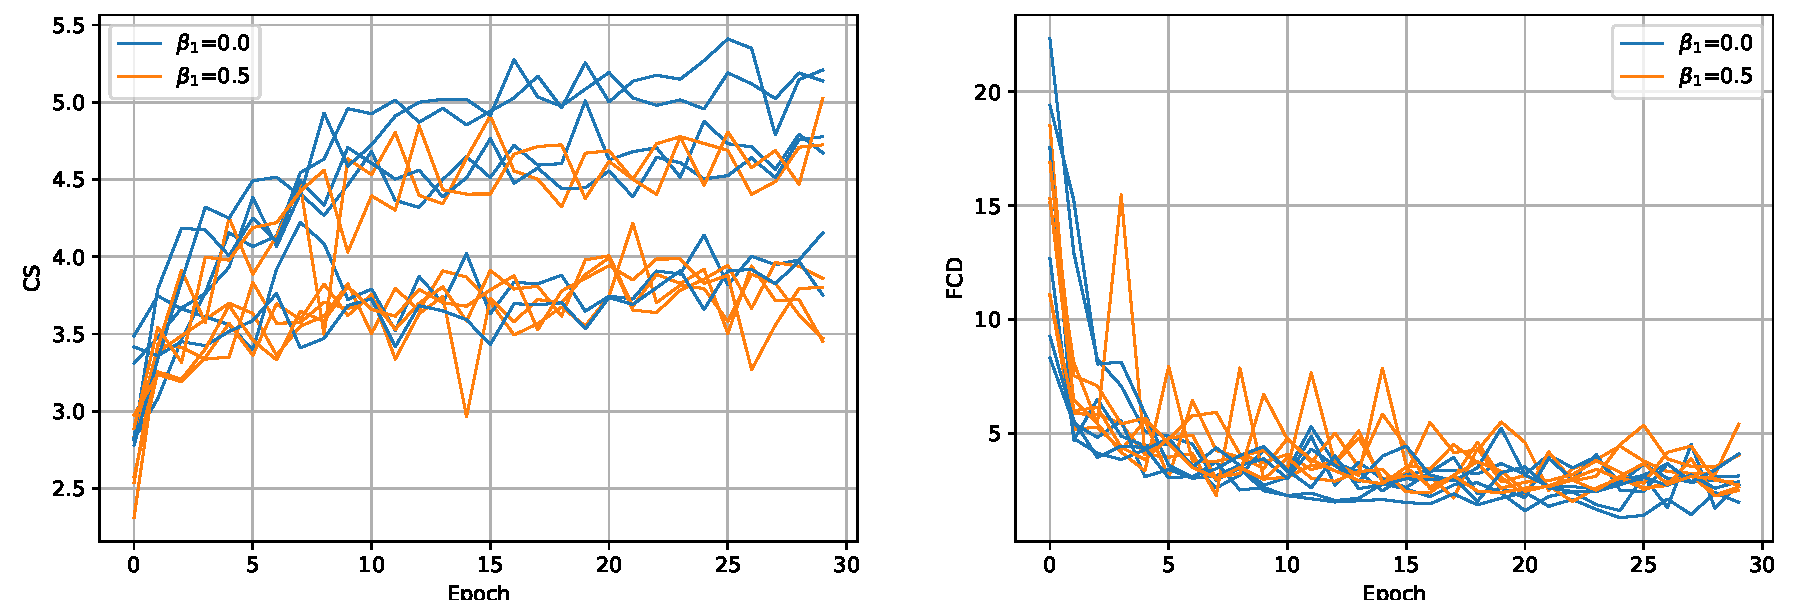
\includegraphics[width=\textwidth]{chapters/Experiments/CGAN/cifar_beta1.pdf}
    \fonte{From the author (2021)}
    \label{fig:cgan_cifar_smoothing}
\end{figure}

The samples produced by the best test (\texttt{$\beta_1$=0.0 UP=TrpConv SMOOTH=0.9}) are shown in \autoref{fig:cgan_cifar_samples}.
\begin{figure}[hbt]
    \centering
    \caption{Samples when training a CGAN on CIFAR-10}
    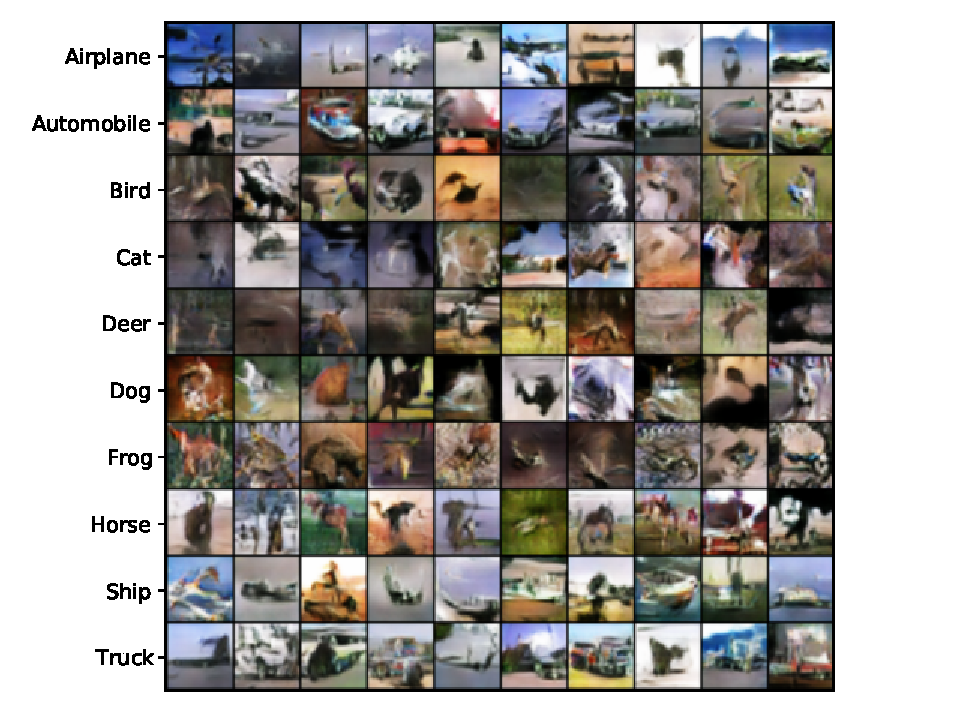
\includegraphics[width=0.65\textwidth]{chapters/Experiments/CGAN/cifar_samples.pdf}
    \fonte{From the author (2021)}
    \label{fig:cgan_cifar_samples}
\end{figure}
